\section{Конструкторская часть}

\noindent
\hspace{1.25cm}
В данном разделе проектируется базы данных для хранения истории деформаций трубчатых поверхностей: описывается структура таблиц с типами данных и ограничениями, рассматриваются хранимые процедуры и триггеры.

\subsection{Проектирование базы данных}

\subsubsection{Таблицы базы данных}

\noindent
\hspace{1.25cm}
Реализуемая база данных включает пять таблиц, соответствующих основным сущностям предметной области: трубка, сечение, точка, сегмент и ребро. Диаграмма базы данных представлена на рисунке~\ref{fig:db_diagram}.

\begin{figure}[H]
\centering
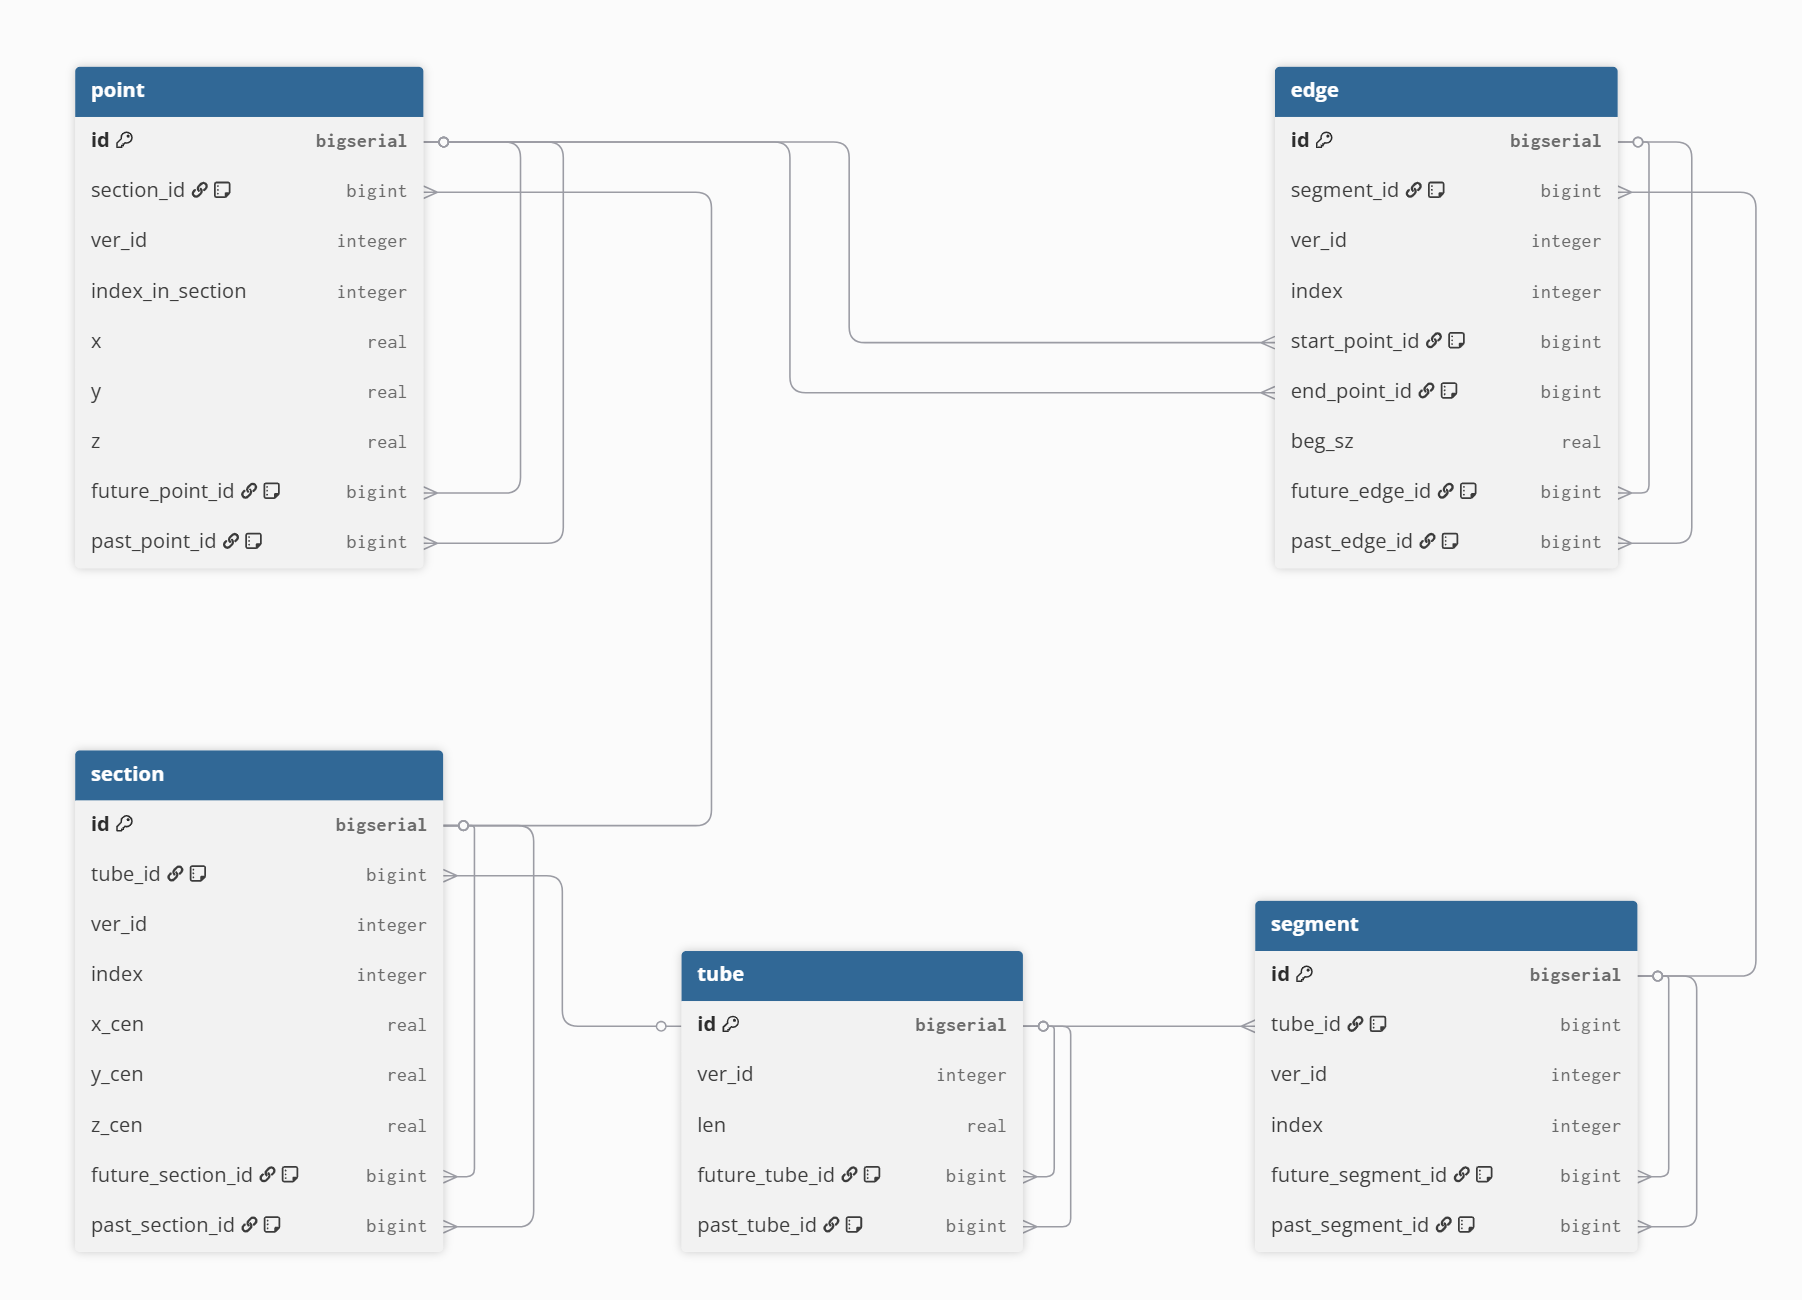
\includegraphics[width=1.0\textwidth]{img/db_diagram.png}
\caption{Диаграмма базы данных}
\label{fig:db_diagram}
\end{figure}


\begin{enumerate}
    \item Таблица \texttt{point} содержит информацию о точках сечений и включает следующие поля:
        \begin{itemize}[leftmargin=\parindent]
            \item \texttt{id}: bigserial --- первичный ключ;
            \item \texttt{section\_id}: bigint --- ссылка на сечение, внешний ключ на таблицу \texttt{section} с каскадным удалением, допускает NULL;
            \item \texttt{ver\_id}: integer --- номер версии точки;
            \item \texttt{index\_in\_section}: integer --- порядковый номер точки в сечении, допускает NULL;
            \item \texttt{x}: real --- координата X точки;
            \item \texttt{y}: real --- координата Y точки;
            \item \texttt{z}: real --- координата Z точки;
            \item \texttt{future\_point\_id}: bigint --- ссылка на следующую версию точки, внешний ключ на таблицу \texttt{point}, допускает NULL;
            \item \texttt{past\_point\_id}: bigint --- ссылка на предыдущую версию точки, внешний ключ на таблицу \texttt{point}, допускает NULL.
        \end{itemize}

    \item Таблица \texttt{section} содержит информацию о сечениях трубки и включает следующие поля:
        \begin{itemize}[leftmargin=\parindent]
            \item \texttt{id}: bigserial --- первичный ключ;
            \item \texttt{tube\_id}: bigint --- ссылка на трубку, внешний ключ на таблицу \texttt{tube} с каскадным удалением;
            \item \texttt{ver\_id}: integer --- номер версии сечения;
            \item \texttt{index}: integer --- порядковый номер сечения в трубке;
            \item \texttt{x\_cen}: real --- координата X центра сечения;
            \item \texttt{y\_cen}: real --- координата Y центра сечения;
            \item \texttt{z\_cen}: real --- координата Z центра сечения;
            \item \texttt{future\_section\_id}: bigint --- ссылка на следующую версию сечения, внешний ключ на таблицу \texttt{section}, допускает NULL;
            \item \texttt{past\_section\_id}: bigint --- ссылка на предыдущую версию сечения, внешний ключ на таблицу \texttt{section}, допускает NULL.
        \end{itemize}

    \item Таблица \texttt{edge} содержит информацию о ребрах, соединяющих точки соседних сечений, и включает следующие поля:
        \begin{itemize}[leftmargin=\parindent]
            \item \texttt{id}: bigserial --- первичный ключ;
            \item \texttt{segment\_id}: bigint --- ссылка на сегмент, внешний ключ на таблицу \texttt{segment} с каскадным удалением;
            \item \texttt{ver\_id}: integer --- номер версии ребра;
            \item \texttt{index}: integer --- порядковый номер ребра в сегменте;
            \item \texttt{start\_point\_id}: bigint --- ссылка на начальную точку ребра, внешний ключ на таблицу \texttt{point} с каскадным удалением;
            \item \texttt{end\_point\_id}: bigint --- ссылка на конечную точку ребра, внешний ключ на таблицу \texttt{point} с каскадным удалением;
            \item \texttt{beg\_sz}: real --- длина ребра;
            \item \texttt{future\_edge\_id}: bigint --- ссылка на следующую версию ребра, внешний ключ на таблицу \texttt{edge}, допускает NULL;
            \item \texttt{past\_edge\_id}: bigint --- ссылка на предыдущую версию ребра, внешний ключ на таблицу \texttt{edge}, допускает NULL.
        \end{itemize}

    \item Таблица \texttt{segment} содержит информацию о сегментах, соединяющих соседние сечения, и включает следующие поля:
        \begin{itemize}[leftmargin=\parindent]
            \item \texttt{id}: bigserial --- первичный ключ;
            \item \texttt{tube\_id}: bigint --- ссылка на трубку, внешний ключ на таблицу \texttt{tube} с каскадным удалением;
            \item \texttt{ver\_id}: integer --- номер версии сегмента;
            \item \texttt{index}: integer --- порядковый номер сегмента в трубке;
            \item \texttt{future\_segment\_id}: bigint --- ссылка на следующую версию сегмента, внешний ключ на таблицу \texttt{segment}, допускает NULL;
            \item \texttt{past\_segment\_id}: bigint --- ссылка на предыдущую версию сегмента, внешний ключ на таблицу \texttt{segment}, допускает NULL.
        \end{itemize}

    \item Таблица \texttt{tube} содержит информацию о трубчатых поверхностях и включает следующие поля:
        \begin{itemize}[leftmargin=\parindent]
            \item \texttt{id}: bigserial --- первичный ключ;
            \item \texttt{ver\_id}: integer --- номер версии трубки;
            \item \texttt{len}: real --- общая длина трубки;
            \item \texttt{future\_tube\_id}: bigint --- ссылка на следующую версию трубки, внешний ключ на таблицу \texttt{tube}, допускает NULL;
            \item \texttt{past\_tube\_id}: bigint --- ссылка на предыдущую версию трубки, внешний ключ на таблицу \texttt{tube}, допускает NULL.
        \end{itemize}
\end{enumerate}


\subsubsection{Хранимые процедуры и функции}

Функция \texttt{calculate\_tube\_length\_on\_segment()} вычисляет длину трубки на основе максимальных значений \texttt{beg\_sz} ребер в каждом сегменте (рисунок~\ref{fig:calculatetubelengthonsegment}).

\begin{figure}[H]
\centering
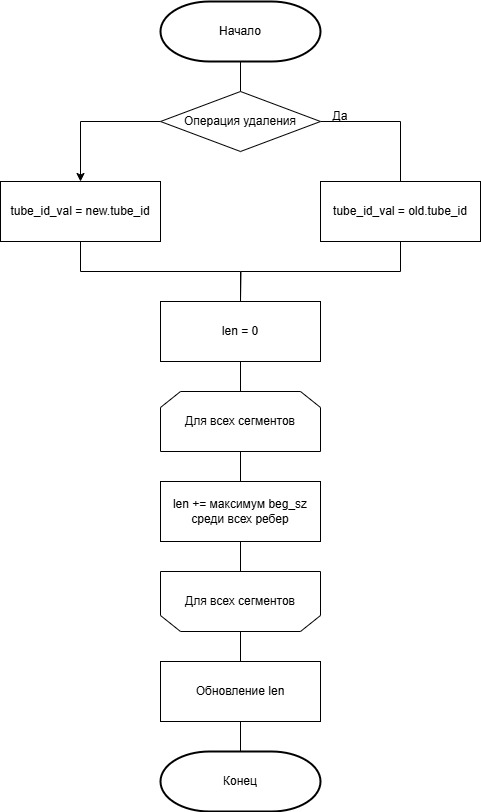
\includegraphics[width=0.5\textwidth]{img/calculate_tube_length_on_segment.jpg}
\caption{Алгоритм функции calculate\_tube\_length\_on\_segment}
\label{fig:calculatetubelengthonsegment}
\end{figure}

Функция \texttt{calculate\_tube\_length\_on\_edge()} выполняет аналогичные вычисления при изменении ребер (рисунок~\ref{fig:calculatetubelengthonedge}). 

\begin{figure}[H]
\centering
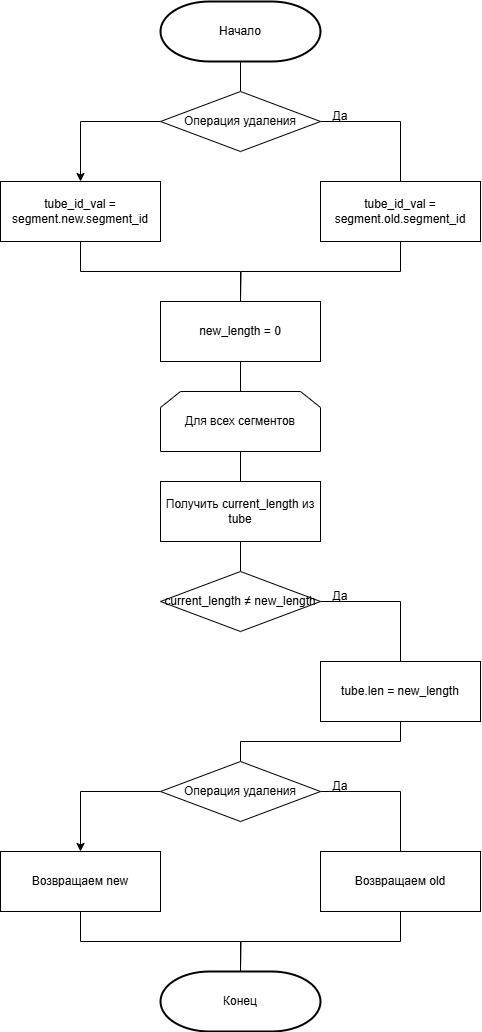
\includegraphics[width=0.5\textwidth]{img/calculate_tube_length_on_edge.jpg}
\caption{Алгоритм функции calculate\_tube\_length\_on\_edge}
\label{fig:calculatetubelengthonedge}
\end{figure}

\subsubsection{Триггеры базы данных}

\noindent
\hspace{1.25cm}
Триггер \texttt{update\_tube\_length\_on\_segment} срабатывает после операций INSERT, UPDATE или DELETE на таблице \texttt{segment} и вызывает функцию \texttt{calculate\_tube\_length\_on\_segment()} для автоматического пересчёта длины трубки при изменении состава сегментов (рисунок~\ref{fig:updatetubelengthonsegment}).

\noindent
\hspace{1.25cm}
Триггер \texttt{update\_tube\_length\_on\_edge} активируется после операций INSERT, UPDATE поля \texttt{beg\_sz} или DELETE на таблице \texttt{edge}, вызывая функцию \texttt{calculate\_tube\_length\_on\_edge()} для поддержания актуальности длины трубки при модификации ребер (рисунок~\ref{fig:updatetubelengthonsegment}).

\begin{figure}[H]
\centering
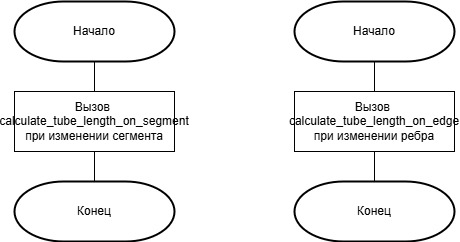
\includegraphics[width=0.7\textwidth]{img/update_tube_length_on_segment.jpg}
\caption{Алгоритм триггера update\_tube\_length\_on\_segment (слева) и триггера update\_tube\_length\_on\_edge (справа)}
\label{fig:updatetubelengthonsegment}
\end{figure}

\subsection{Вывод}

\noindent
\hspace{1.25cm}
В данном разделе была спроектирована база данных для хранения истории деформаций трубчатых поверхностей: описаны пять таблиц со спецификацией типов данных и ограничений целостности, рассмотрены основные хранимые процедуры, функции и триггеры.

\newpage